\chapter*{Anhang}\addcontentsline{toc}{chapter}{Anhang}\setcounter{chapter}{1}


\begin{figure}
	\centering
	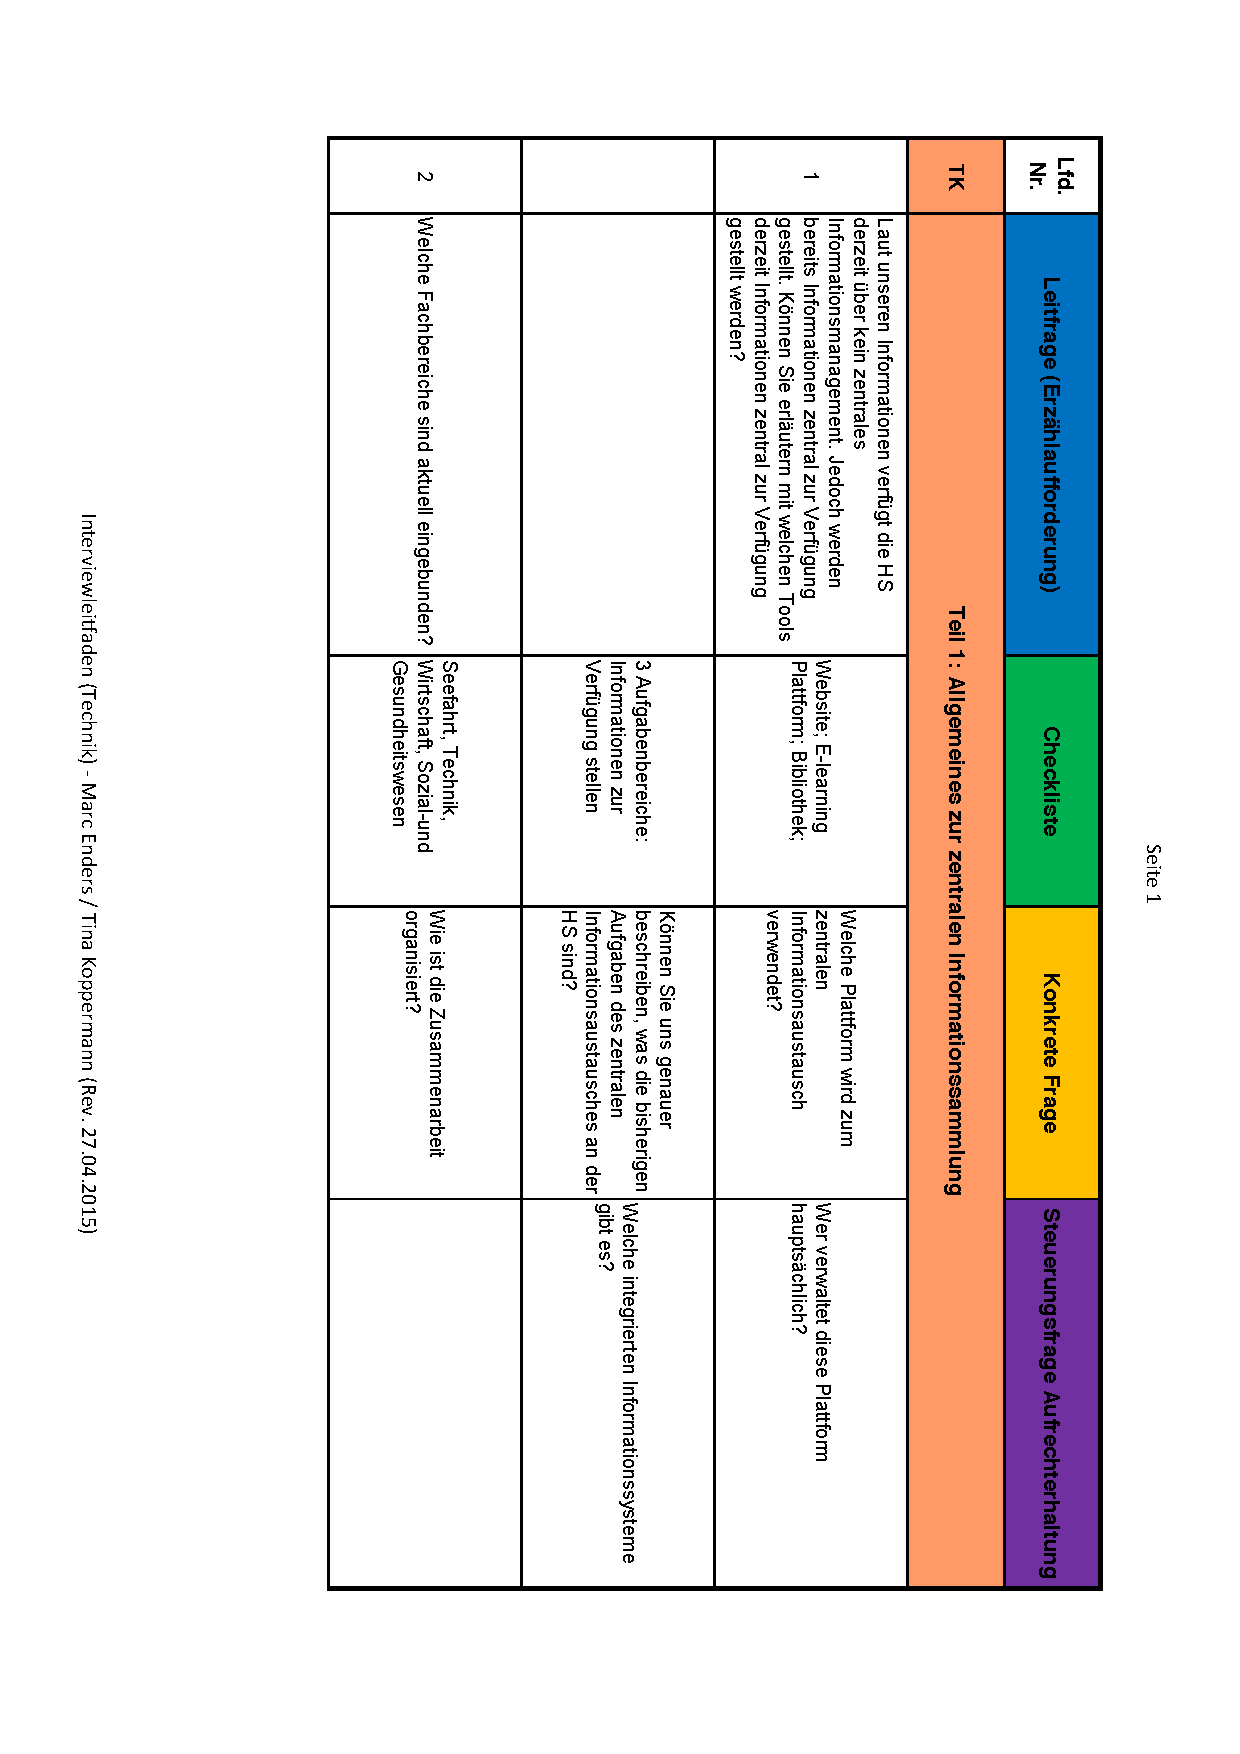
\includegraphics[width=18cm]{kapitel/anhang/Interviewleitfaden_1}
\end{figure}

\begin{figure}
	\centering
	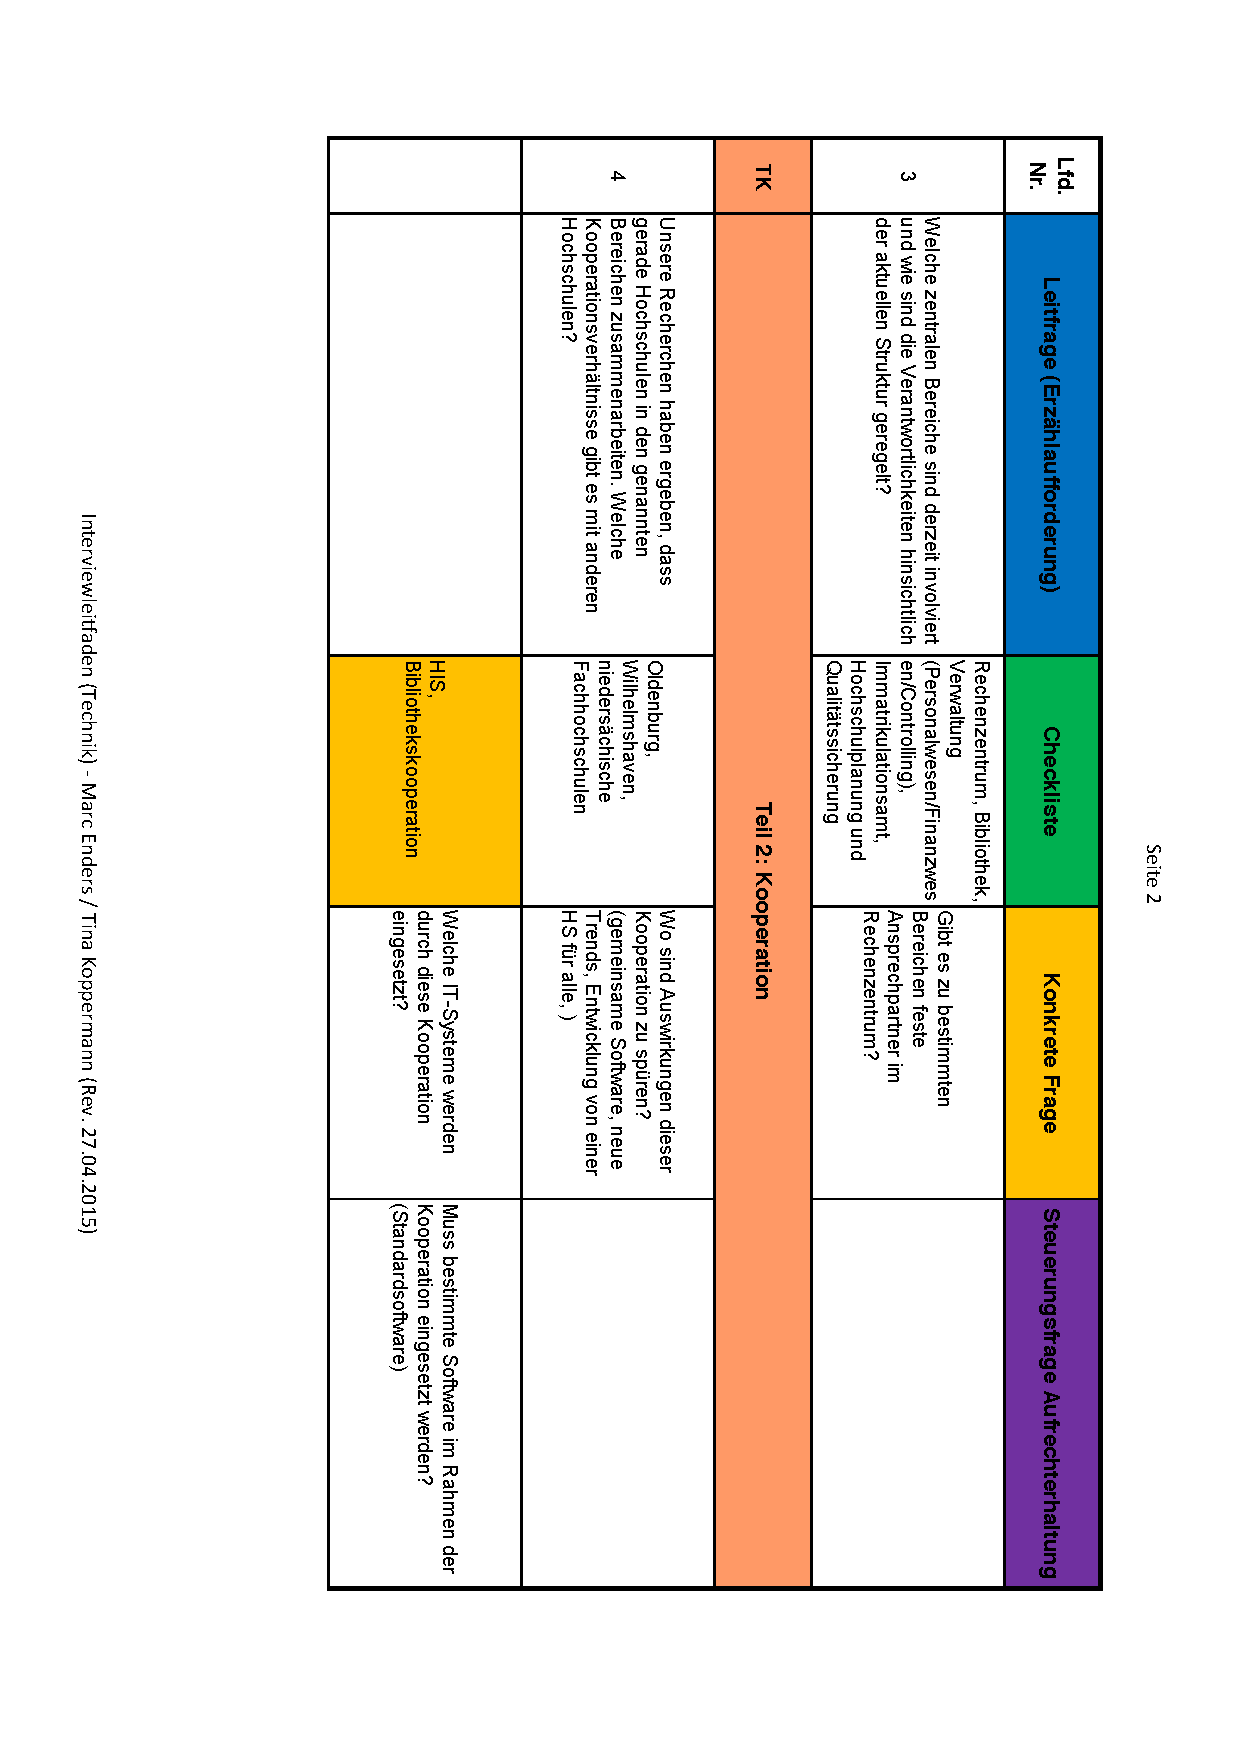
\includegraphics[width=18cm]{kapitel/anhang/Interviewleitfaden_2}
\end{figure}

\begin{figure}
	\centering
	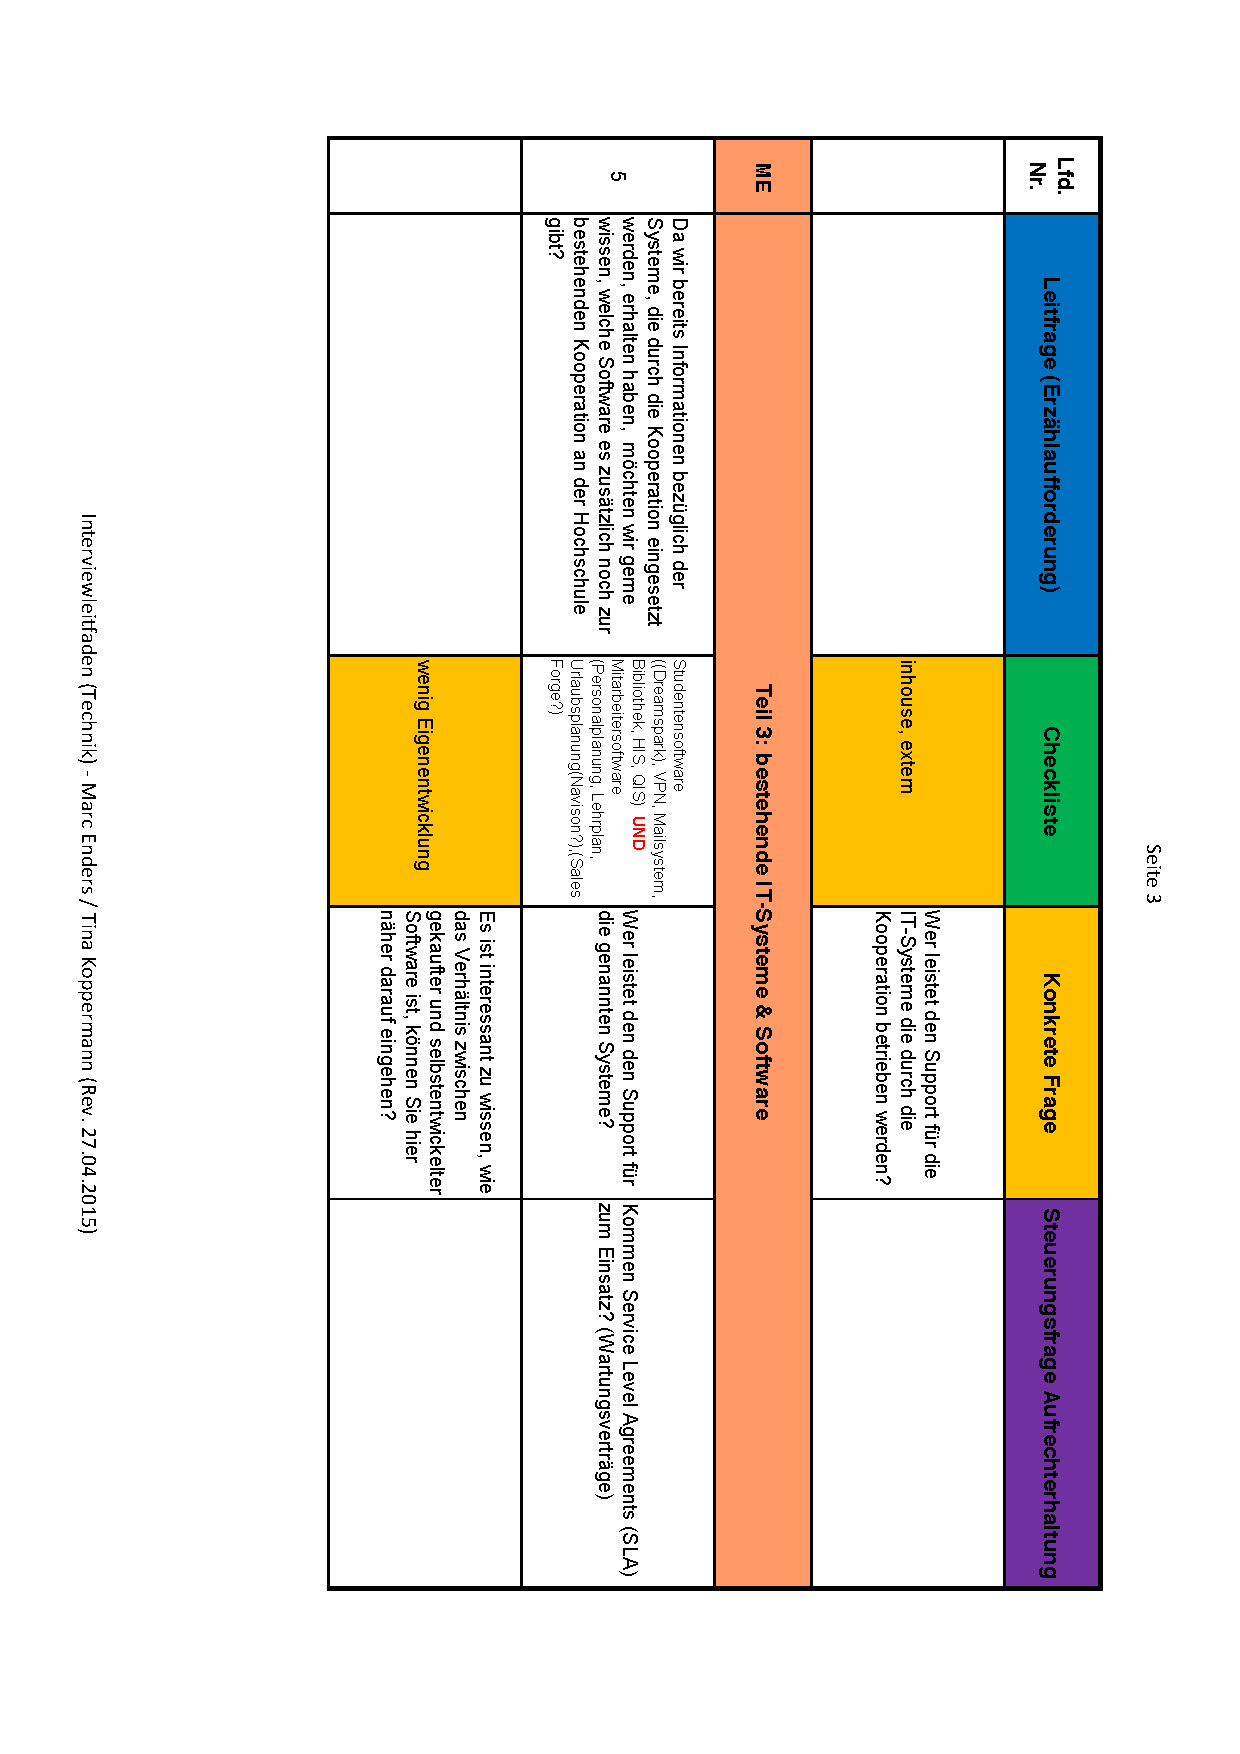
\includegraphics[width=18cm]{kapitel/anhang/Interviewleitfaden_3}
\end{figure}

\begin{figure}
	\centering
	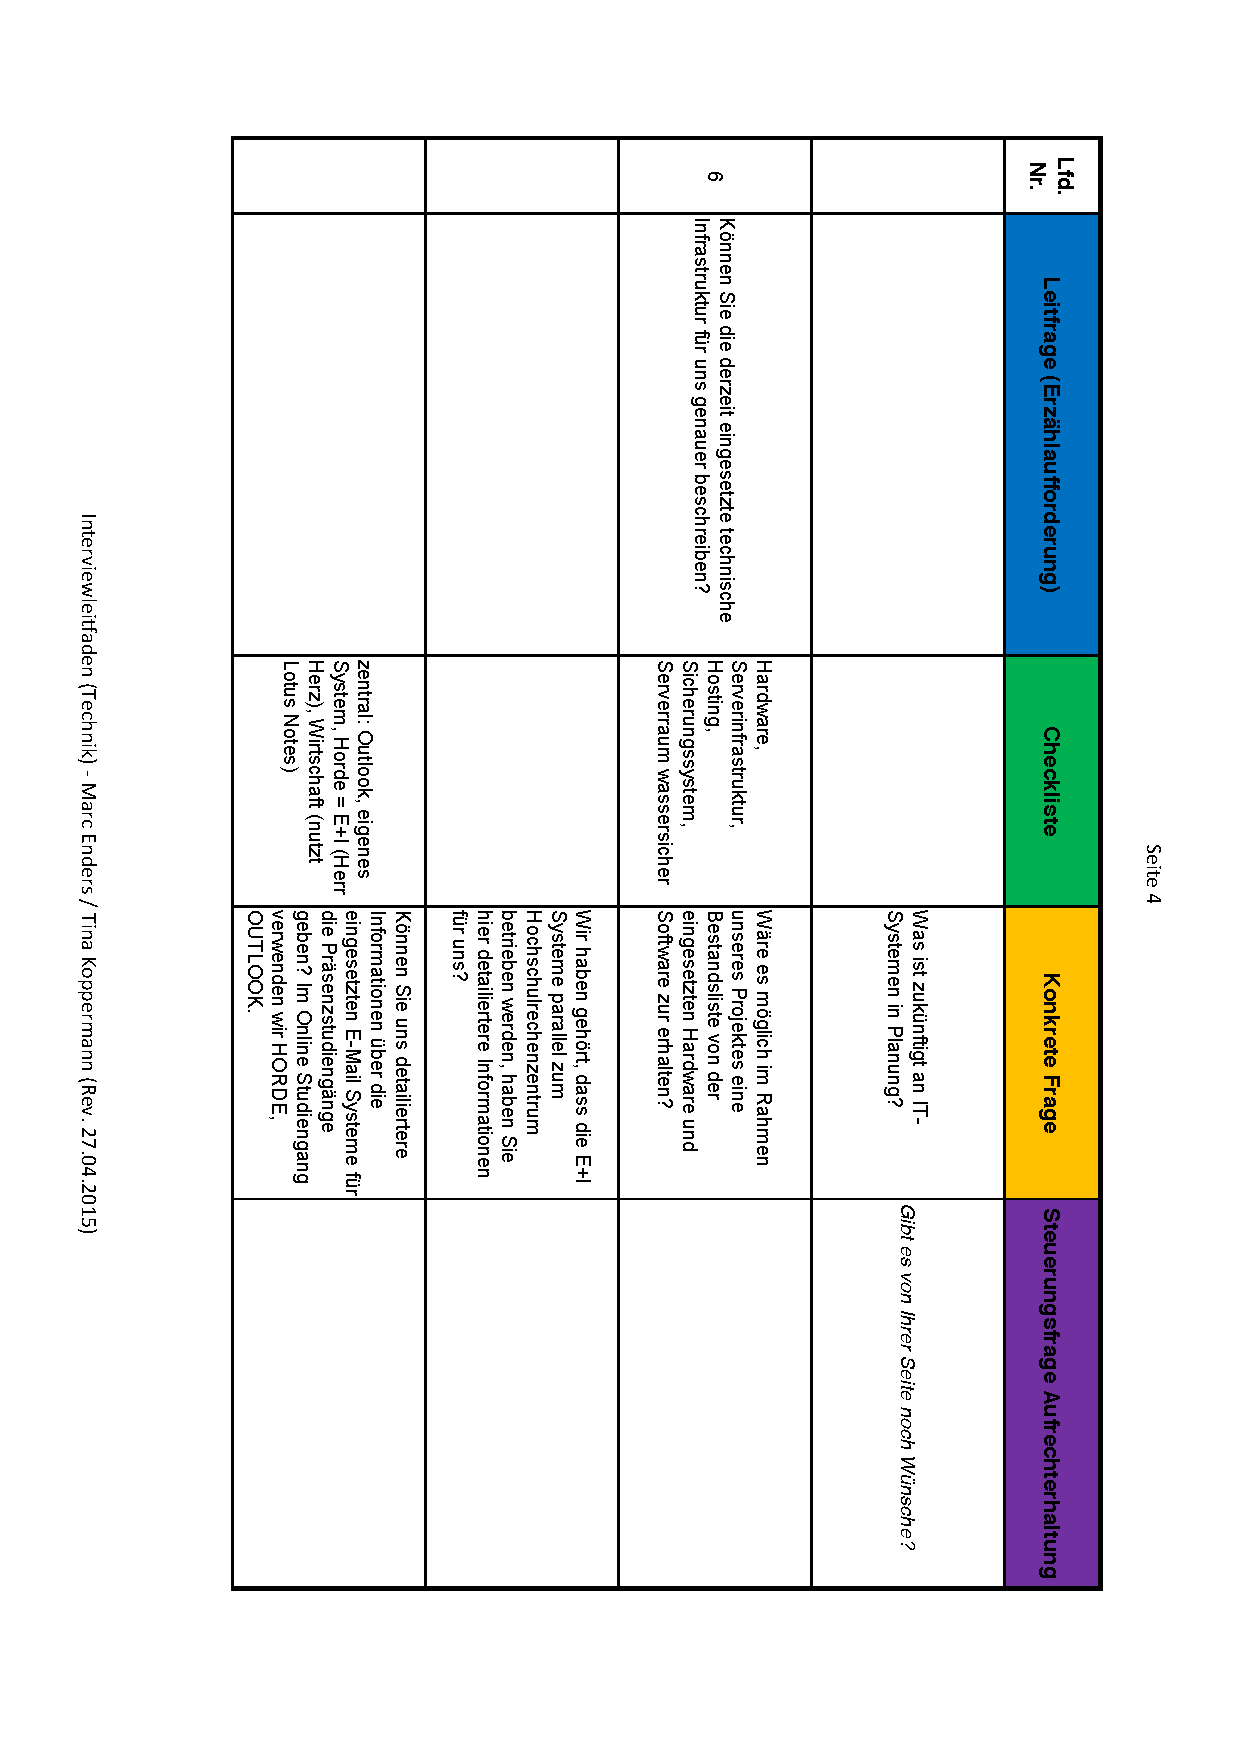
\includegraphics[width=18cm]{kapitel/anhang/Interviewleitfaden_4}
\end{figure}

\begin{figure}
	\centering
	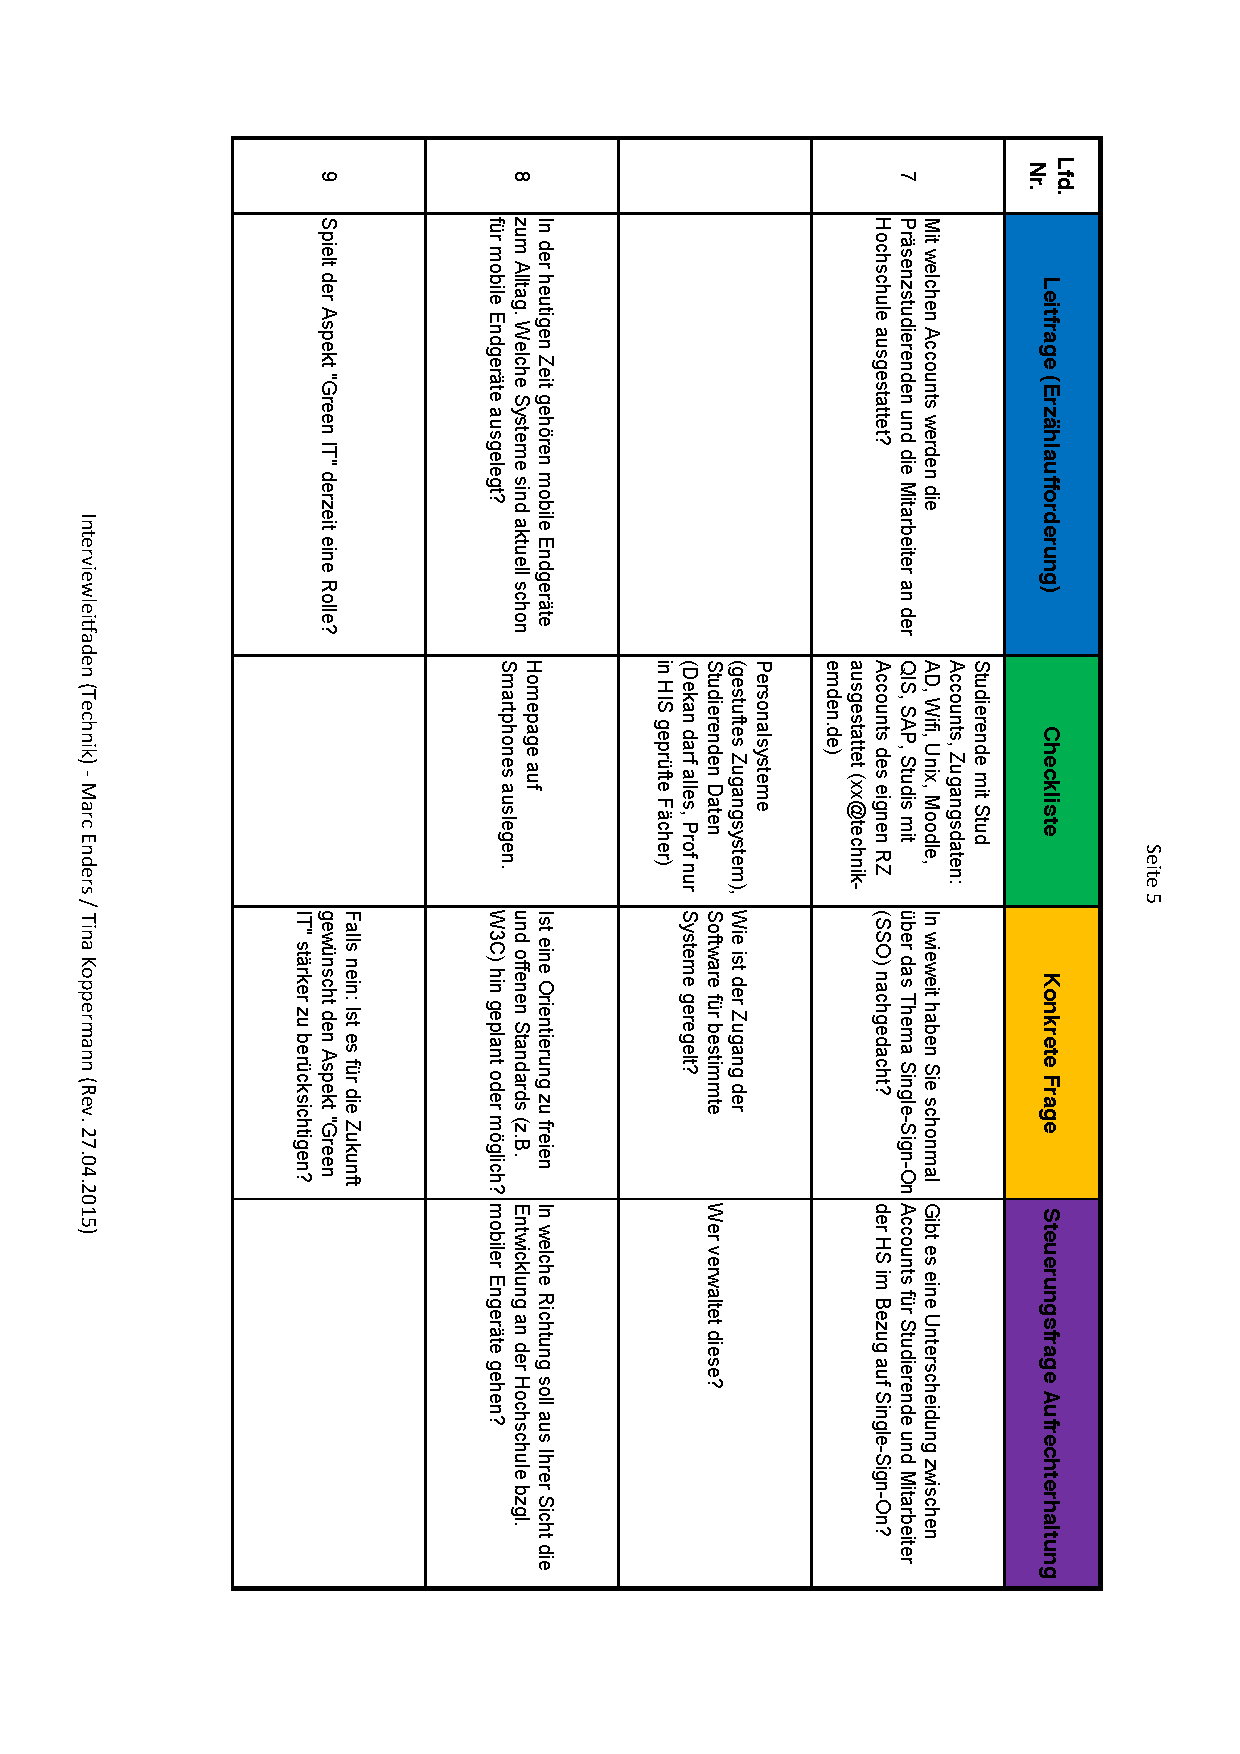
\includegraphics[width=18cm]{kapitel/anhang/Interviewleitfaden_5}
\end{figure}

\begin{figure}
	\centering
	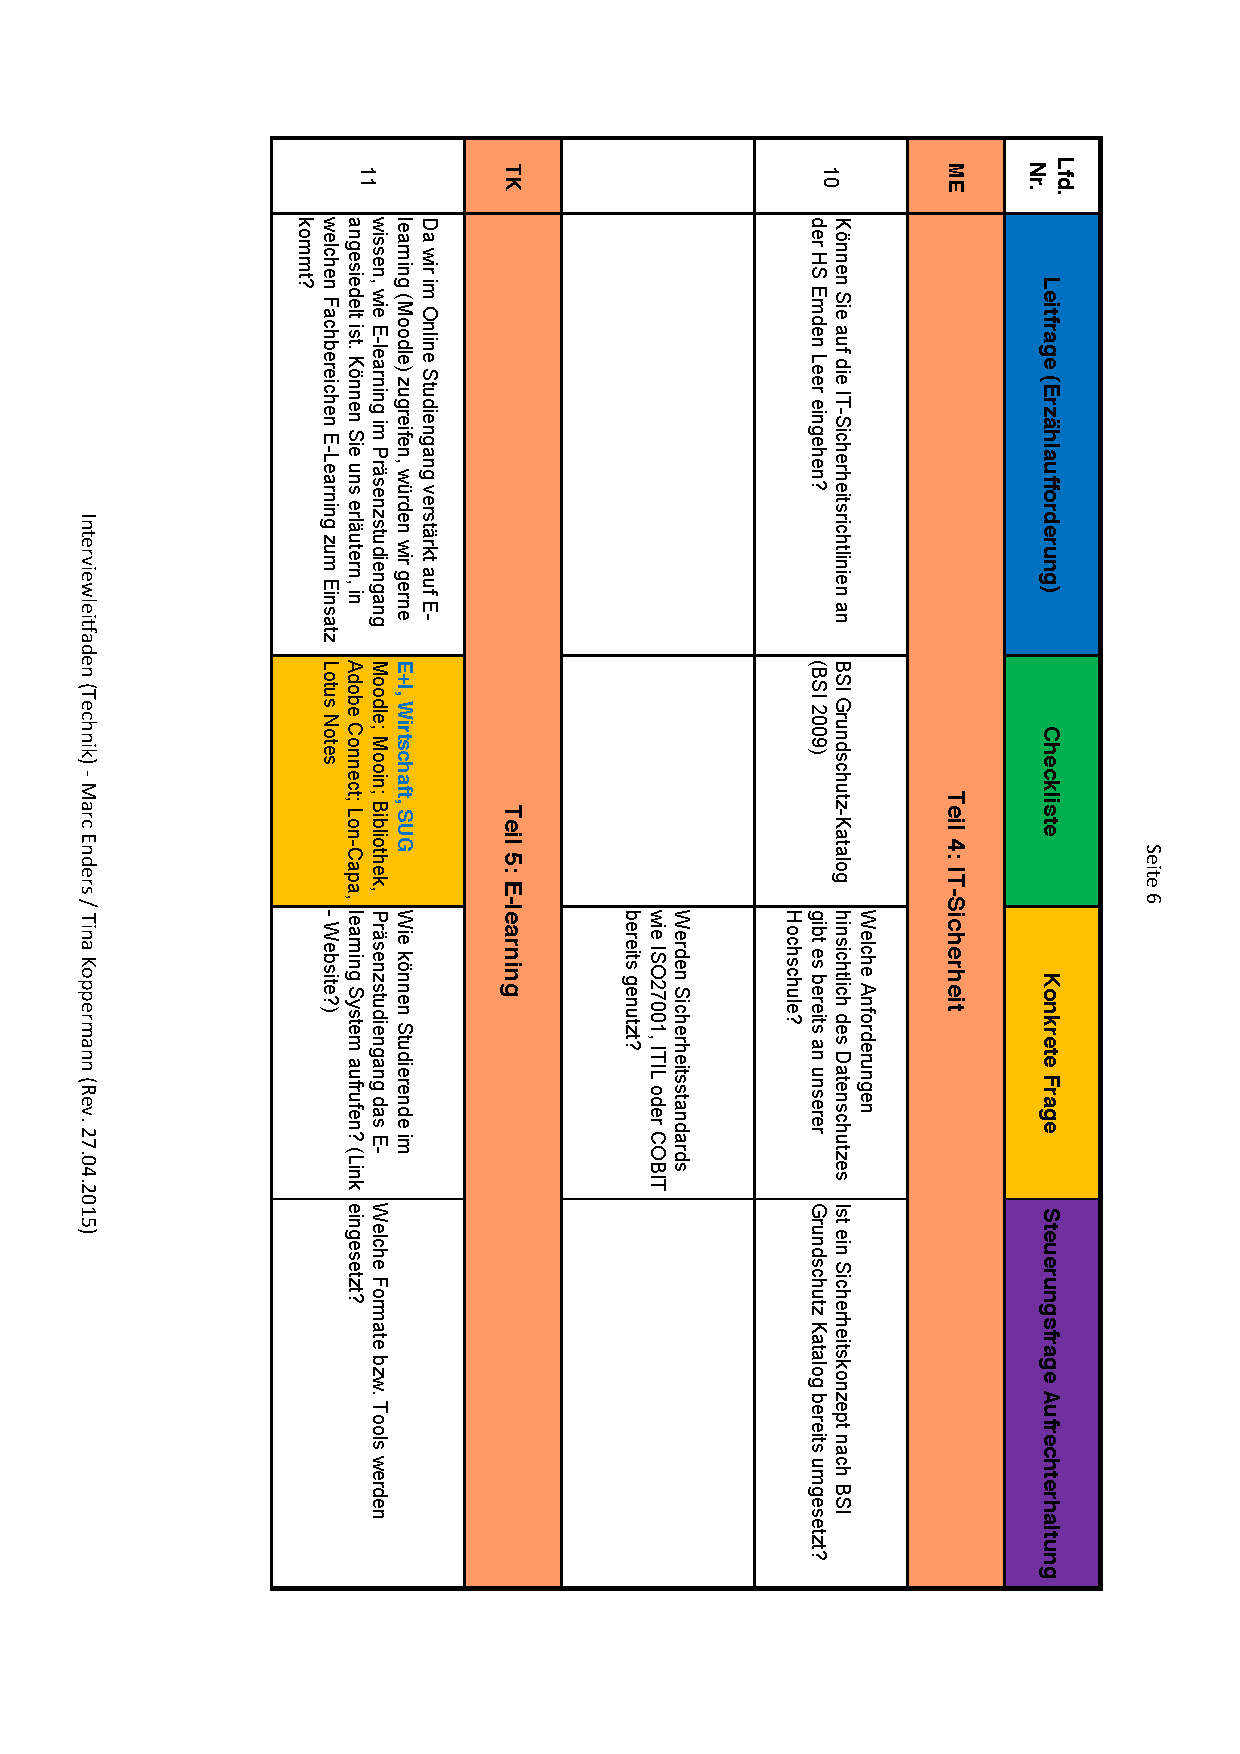
\includegraphics[width=18cm]{kapitel/anhang/Interviewleitfaden_6}
\end{figure}

\begin{figure}
	\centering
	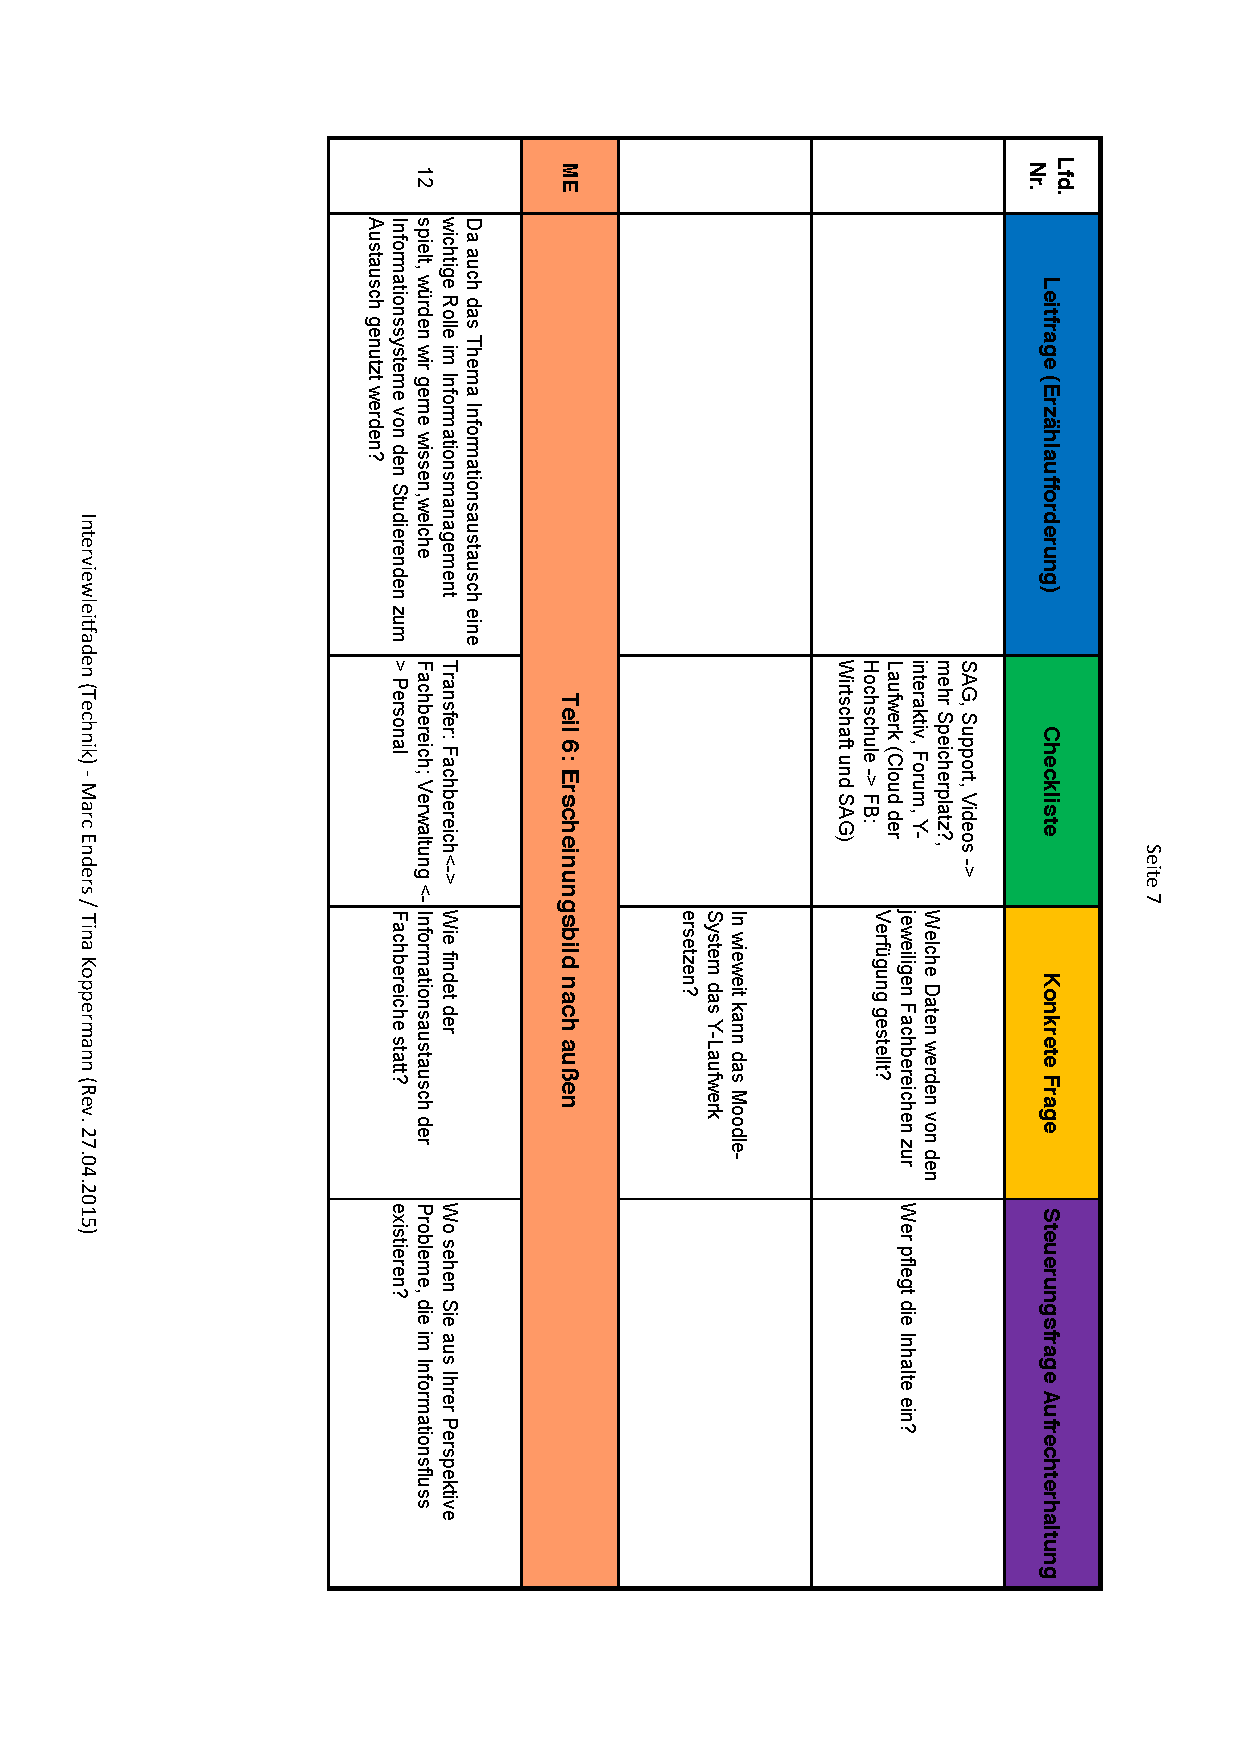
\includegraphics[width=18cm]{kapitel/anhang/Interviewleitfaden_7}
\end{figure}

\begin{figure}
	\centering
	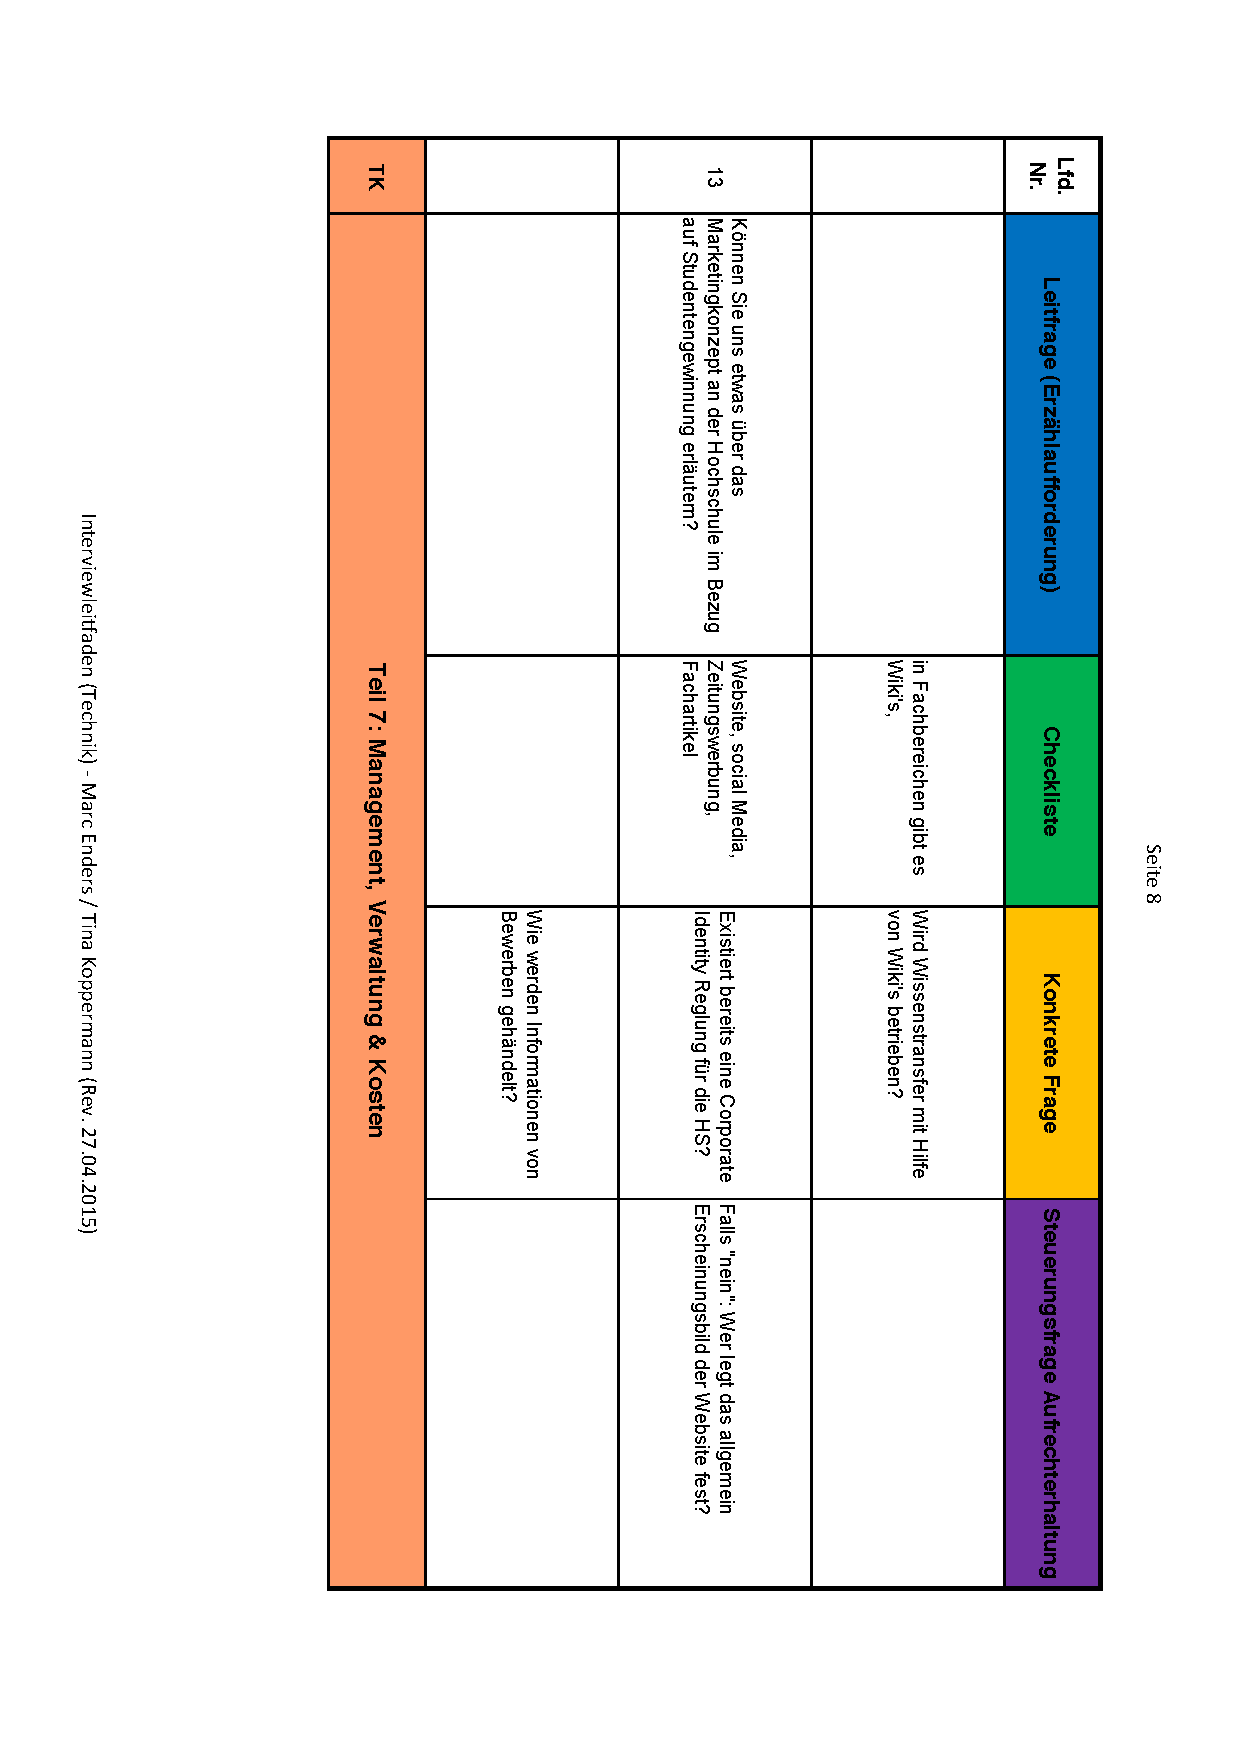
\includegraphics[width=18cm]{kapitel/anhang/Interviewleitfaden_8}
\end{figure}

\begin{figure}
	\centering
	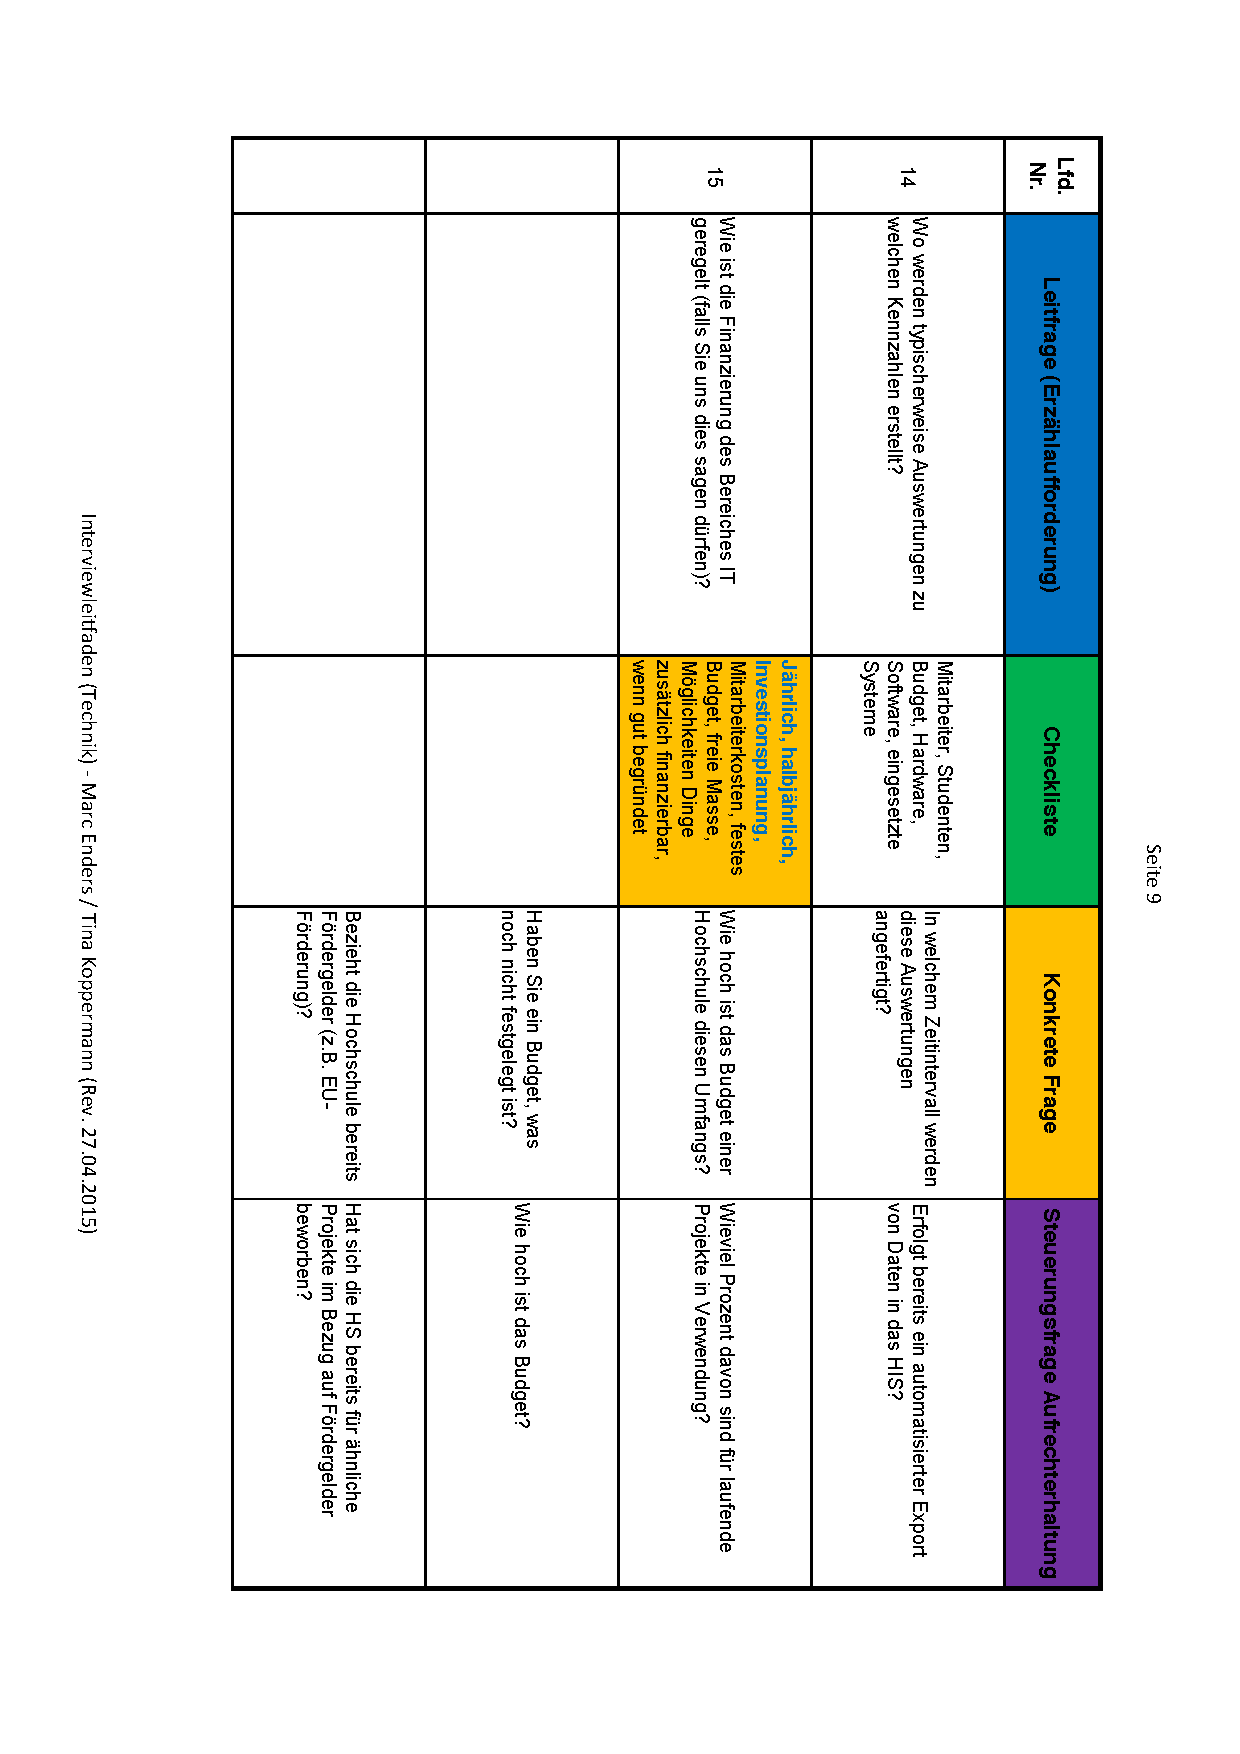
\includegraphics[width=18cm]{kapitel/anhang/Interviewleitfaden_9}
\end{figure}

\begin{figure}
	\centering
	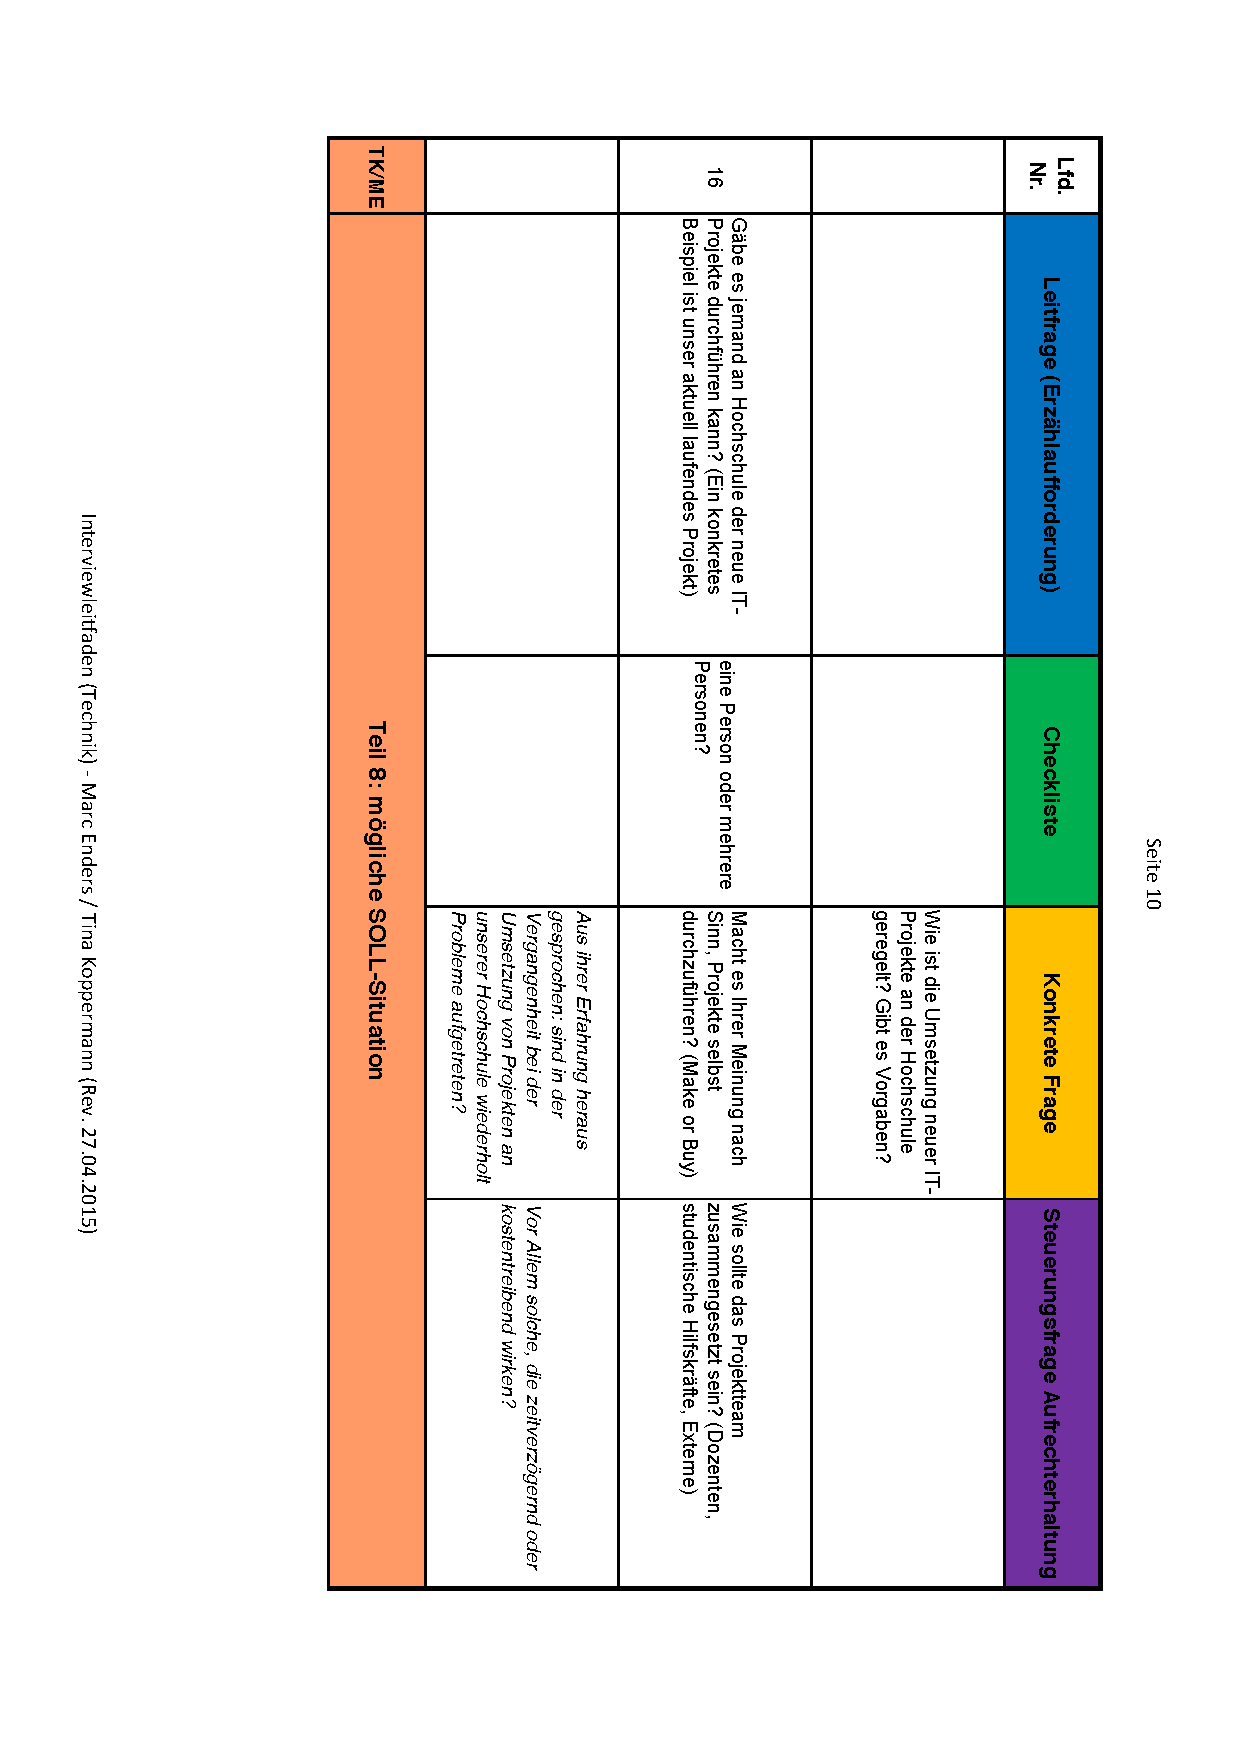
\includegraphics[width=18cm]{kapitel/anhang/Interviewleitfaden_10}
\end{figure}

\begin{figure}
	\centering
	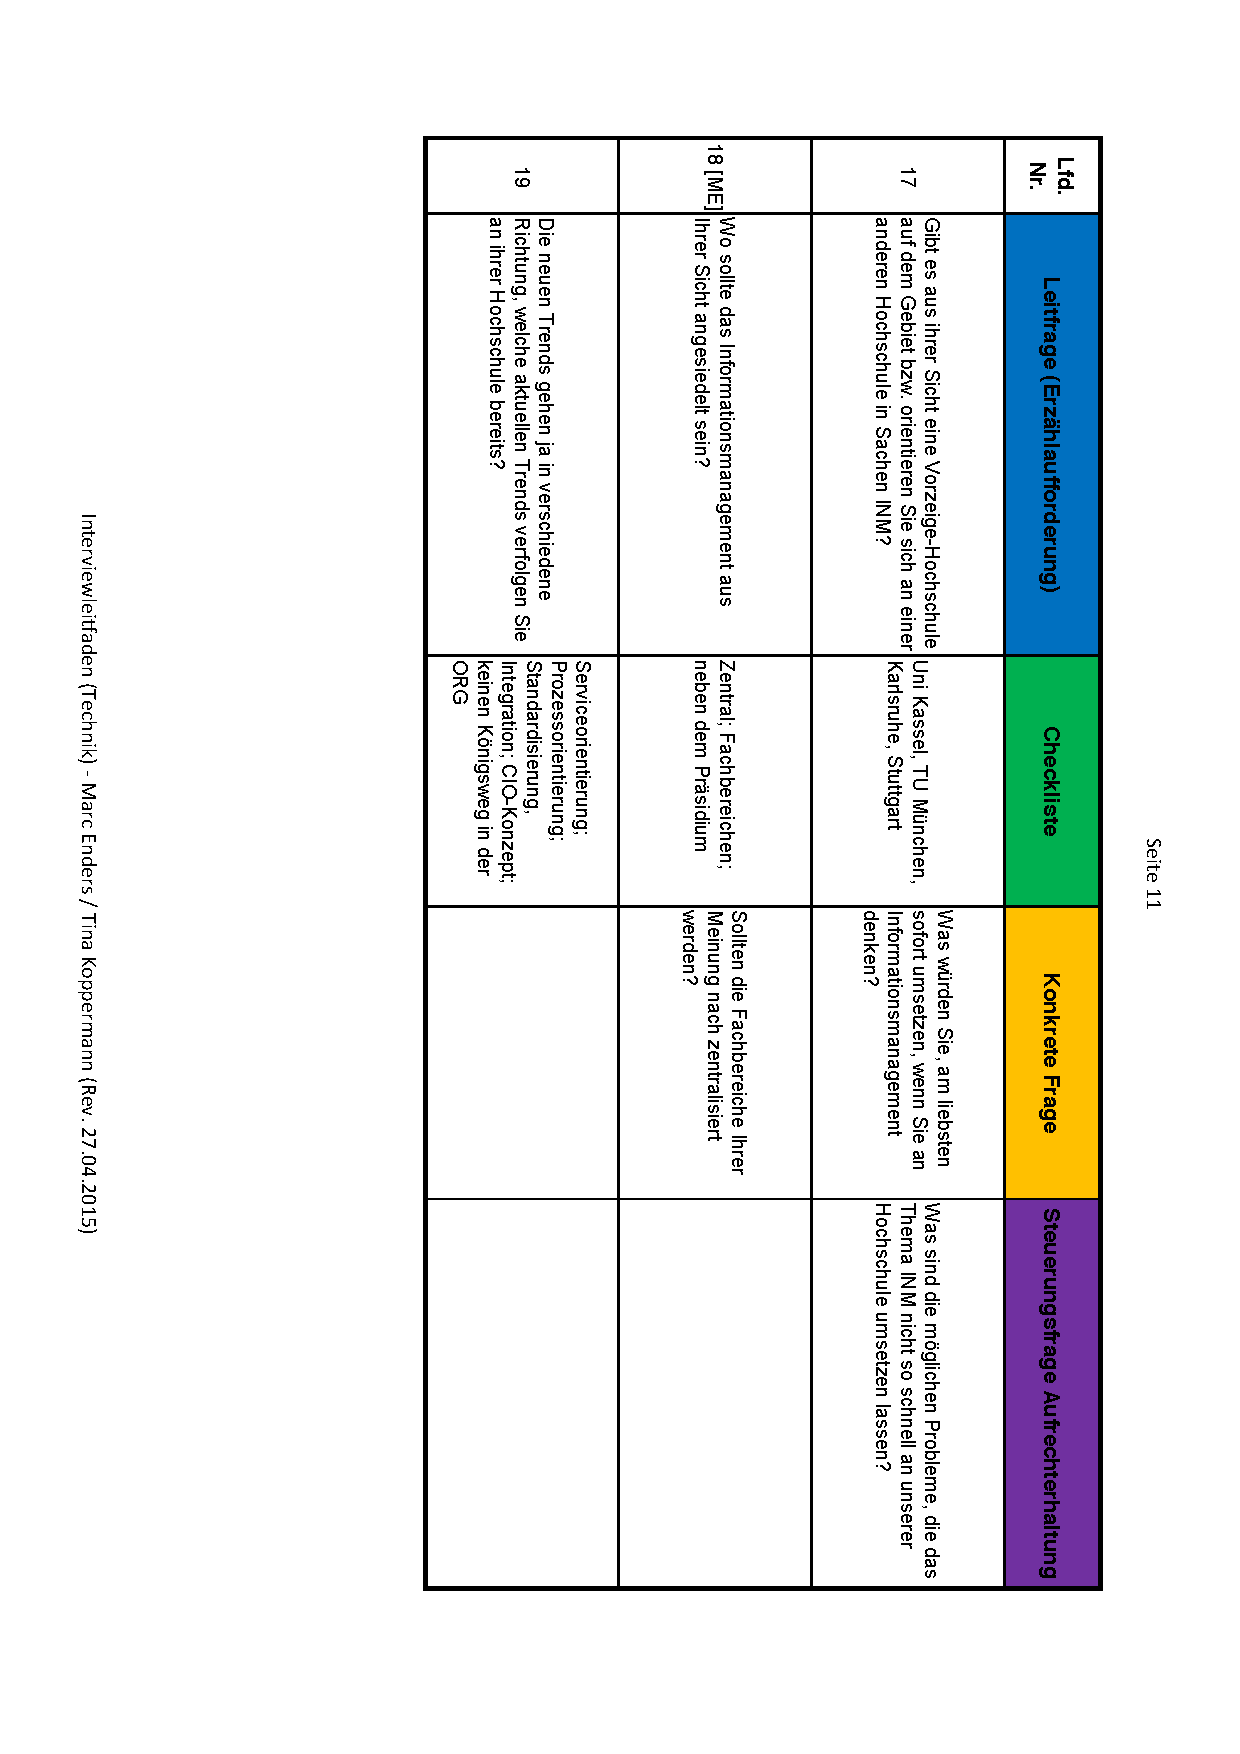
\includegraphics[width=18cm]{kapitel/anhang/Interviewleitfaden_11}
\end{figure}

%\begin{landscape}
    \begin{figure}
	    \centering
	    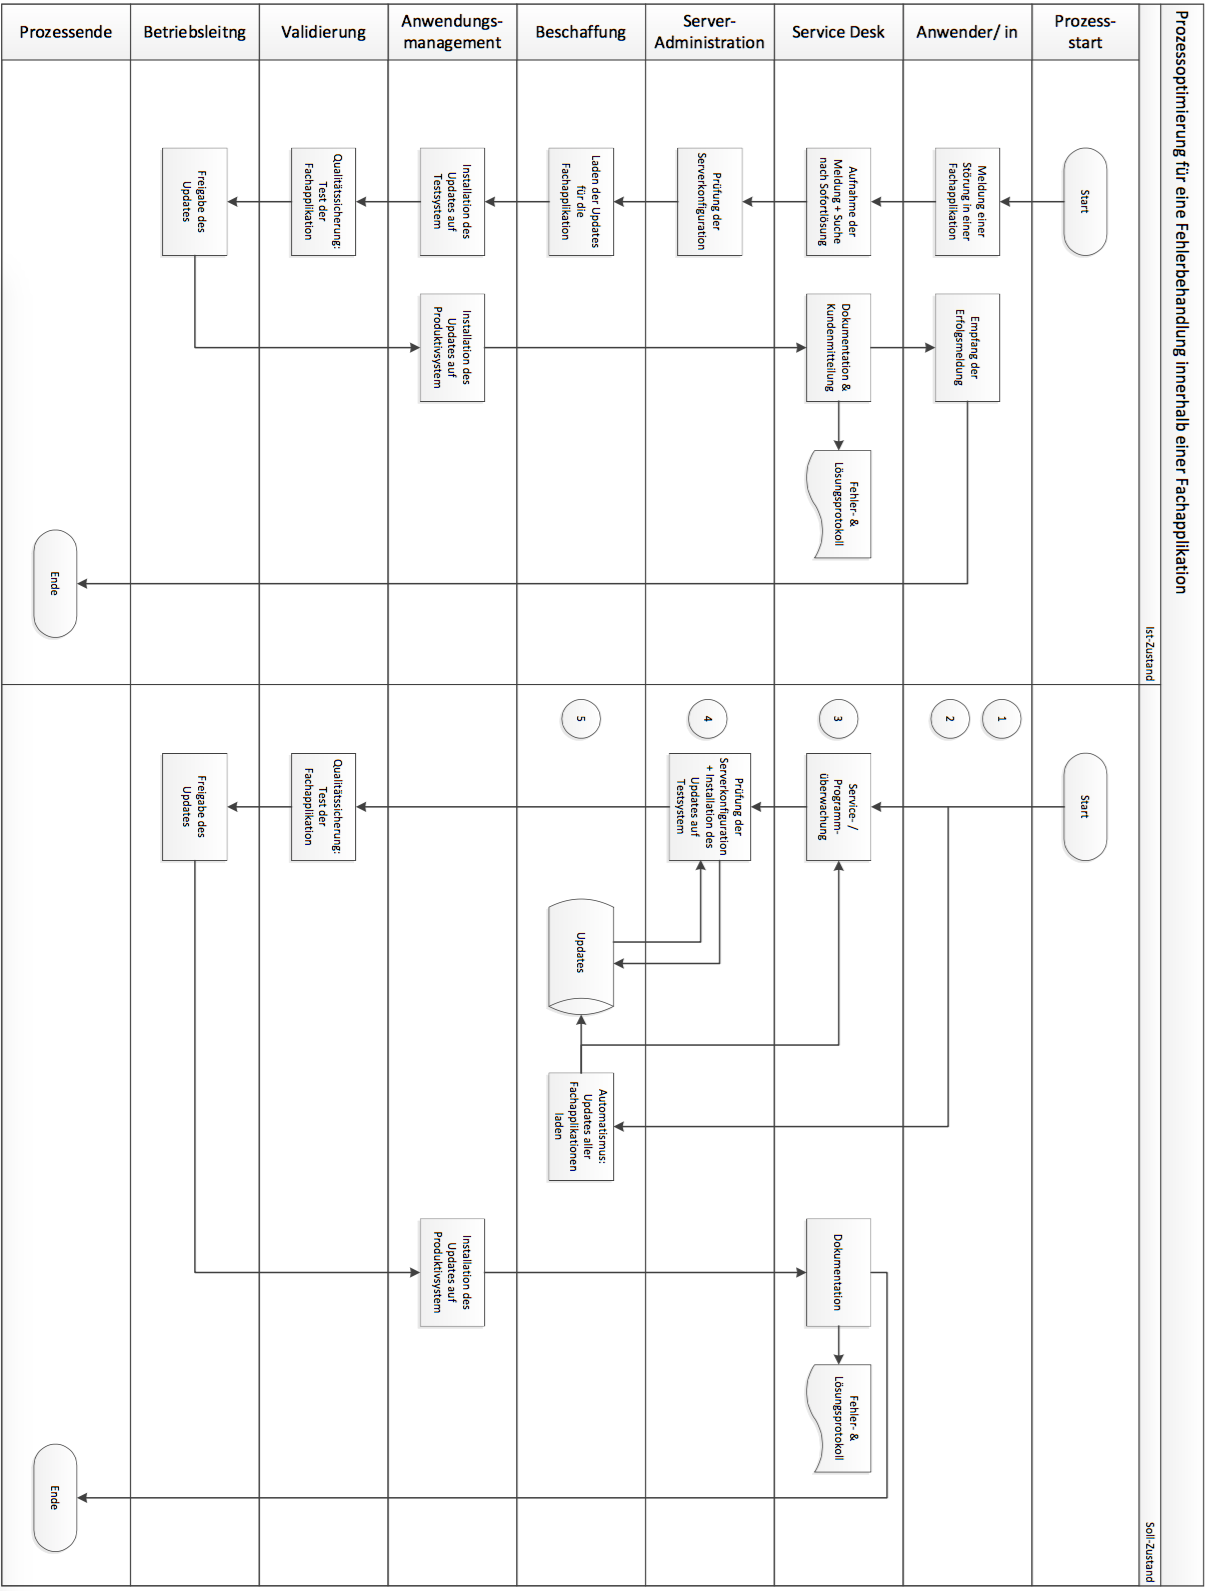
\includegraphics[width=16cm]
	    {kapitel/anhang/prozessoptimierung_gesamt_hoch}
	    \caption*{Prozessoptimierung gesamt}
	    \label{fig_prozessoptimierung_gesamt}
    \end{figure}
%\end{landscape}